\section{Problem formulation}

The detailed topography of the seafloor relevant for landing of underwater vehicles can be rough and vary abruptly on scales that are too small to be captured by traditional ship based acoustic multibeam systems. Seafloor in areas of interest can have complex and abruptly varying terrains, as seen in Fig.~\ref{f:mehul1} which illustrates scenes from a manganese crust survey at No.$5$ Takuyo seamount \cite{Thornton2013l}. 

\begin{figure}[!ht]
\centering
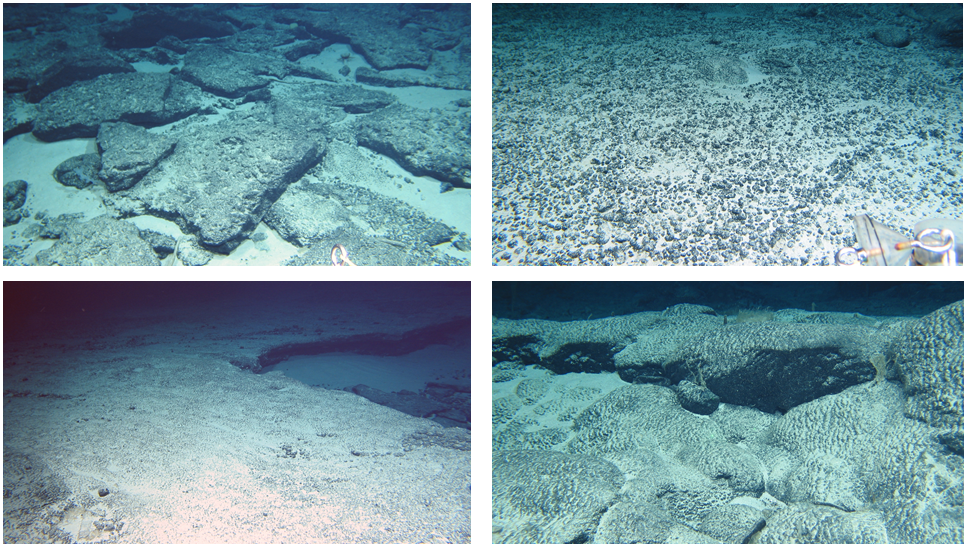
\includegraphics[width=5.5in]{./images/mehul1.png}
\caption{Different seafloor terrain at No.$5$ Takuyo seamount. Clockwise, from top left: Broken slabs in sand, nodules, pillowy crusts and continuous flat crusts}
\label{f:mehul1}
\end{figure}

These prohibit landing simply at random locations and requires intelligent choice of landing sites. However, the large localization uncertainty \cite{Masmitja2016} associated with deep sea operations means that landing sites determined prior to deployment cannot be reached with sufficient navigational accuracy. Therefore, the AUV should have capability to identify landing sites during the survey. This requires it to be equipped with a mapping system capable of generating bathymetry with sufficiently high resolution, such as those based on light sectioning \cite{Inglis2012} \cite{Nishida2016}. While landing site detection for aerial vehicles has been previously demonstrated in \cite{Desaraju2014} \cite{Sharp2001}, conditions essential for safe landing with a stable footing in underwater environments need to be investigated. Simulations for control, navigation and dynamics of AUVs with landing capabilities have been reported in \cite{Wang2007}\cite{Du2012}. However, these previous works do not develop the intelligence necessary for an AUV to identify areas where it can land safely. This identifies need for an algorithm to perform real-time analysis of seafloor bathymetry to detect landing sites based on the terrain and geometry of the AUV. The use of Fourier analysis for seafloor terrain segmentation and 3D alignment in post-survey processing has been previously demonstrated  in \cite{Douillard2012}\cite{Douillard2013}.  Other methods for surface classification using wavelets \cite{Bhandari2007} have also been demonstrated before but have not been applied earlier to landing site identification. Early works by our group demonstrated a landing algorithm using Fourier analysis to separate flat ground surface from objects on the seafloor \cite{Sangekar2010c}. The algorithm rejected all objects as non-landing areas without analyzing the possibility of landing on objects depending on their size. Also, only extremely flat areas were considered for landing and detailed analysis of landing on slopes was not performed. This work builds on our previous work and develops a complete comprehensive framework for landing including the a design of an underwater vehicle. 
